\chapter{Ergebnis}
\label{chap:ergebnis}

In diesem Kapitel werden die Entscheidungssysteme FSM, BT und GOAP aus der Erfahrung durch die Implementierung \autocite{oleg}, Benchmarks, wissenschaftlicher Literatur verglichen und folglich bewertet.

Der Vergleich wird sich auf die folgenden Punkte fokussieren: Erlernbarkeit, Umsetzung, Skalierbarkeit, Debugging, Performance und Speicherverbrauch. 

F\"{u}r den Vergleich der Performance und Speicherverbrauch werden Ergebnisse von Benchmarks einbezogen.

\section{Ergebnisse der Implementierung}

In Kapitel \ref{chap:loesungskonzept} wird das L\"{o}sungskonzept beschrieben. Dort wird erl\"{a}utert, dass die Bewertung der Entscheidungssysteme auf wissenschaftlicher Literatur sowie praktischen Erfahrungen basiert. Letztere ergeben sich aus der Implementierung der drei Entscheidungssysteme in einem spezifischen Szenario und flie\ss{}en in die abschlie\ss{}enden Vergleich ein. Die Implementierung des Szenarios wird im Kapitel \ref{chap:implementierung lk} beschrieben.


\subsection{Erlernbarkeit}
\label{chap:erlernbarkeit}

Die Erlernbarkeit beschreibt, wie komplex es f\"{u}r Entwickler ist, das jeweilige Entscheidungssystem zu verstehen und anzuwenden. Sie h\"{a}ngt von mehreren Faktoren ab. Dazu geh\"{o}rt die Verst\"{a}ndlichkeit der Konzepte, die Verf\"{u}gbarkeit von Dokumentationen sowie die notwendigen Vorkenntnisse f\"{u}r die Nutzung.

%FSM
Die FSM ist leicht verst\"{a}ndlich. Sie wird h\"{a}ufig als Einf\"{u}hrungsbeispiel in die Game-AI Entscheidungssysteme genommen, wie es in vielen Fachb\"{u}chern, wie \autocite{AIgames, aiag}, zur Game-AI ersichtlich ist. Es gibt gen\"{u}gend Internet Quellen, die eine FSM Implementierung dokumentieren. Haupts\"{a}chlich werden Kenntnisse \"{u}ber endliche Automaten ben\"{o}tigt. Im Vergleich zu den anderen Entscheidungssystemen ist sie am einfachsten zu erlernen.

%BT
Aufgrund der verschiedenen Task-Kategorien ist der BT anspruchsvoller in der Anwendung und Einf\"{u}hrung als die FSM. Kenntnisse in der Graphentheorie, insbesondere \"{u}ber gerichtete Graphen, sind f\"{u}r das Verst\"{a}ndnis eines BT von Vorteil. Sie hat ebenfalls viele Dokumentationen zur Implementierung.

%GOAP
Mit dem dynamischen System kommt die Komplexit\"{a}t der Funktionsweise. GOAP wird im Gegensatz zu den anderen beiden Entscheidungssysteme f\"{u}r fortgeschrittene Entwickler empfohlen. Kenntnisse im Bereich von Graphentheorie und Suchalgorithmen k\"{o}nnen das Verst\"{a}ndnis und die Nutzung von GOAP jedoch erheblich erleichtern. In Bezug auf Dokumentation und verf\"{u}gbare Bibliotheken weist GOAP M\"{a}ngel auf. Wie bereits im Kapitel \ref{chap:goap sota} erl\"{a}utert, fordern Studien wie \autocite{sielicki2018adaptation} eine st\"{a}rkere Verbreitung von Dokumentationen und Bibliotheken f\"{u}r GOAP. Im Vergleich zu den anderen Entscheidungssystemen gibt es zu GOAP deutlich weniger Dokumentation.


\subsection{Umsetzung}
\label{chap:umsetzung}

Bei der Umsetzung liegt der Fokus auf der praktischen Umsetzung des Entscheidungssystems in der Game-Engine Godot. Dabei wird betrachtet, wie aufwendig die Implementierung der Funktionsweise und Architektur des Entscheidungssystems ist sowie das designen der NPCs.

%FSM
Die FSM ist als Ad-Hoc-Authoring Methode ein statisches Entscheidungssystem und in Godot unkompliziert zu implementieren. Die Architektur besteht dabei aus einer Knoten Klasse und einer Koordinaten Klasse. Einen Knoten zu erstellen und diesen mit Aktions Komponenten zu erg\"{a}nzen ist einfach. Doch mit der gr\"{o}\ss{}e der Komplexit\"{a}t eines NPC steigt der Aufwand die FSM instandzuhalten, da mit der Anzahl an Aktionen die Anzahl der Knoten im Graphen steigen.

%BT
Auch der BT ist als Ad-Hoc-Authoring Methode ein statisches Entscheidungssystem und in Godot unkompliziert zu implementieren. Im Vergleich zur FSM hat er aber durch die verschiedenen Task-Typen eine komplexere Architektur. Die Architektur ist aber unaufwendig zu realisieren und man hat durch die verschiedenen Kategorien der Tasks die M\"{o}glichkeit komplexere NPC Verhalten umzusetzen. Dennoch wird der BT als zu statisch empfunden. \autocite{aiag} Zudem m\"{u}ssen Entwickler viel Zeit darauf verwenden, passende BT-Knoten zu erstellen und sie mit den richtigen Verhaltensweisen verkn\"{u}pfen. \autocite{Schwab2021} Wie bereits in den zuvor erl\"{a}uterten Studien aus dem Kapitel \ref{chap:bt sota}, kann die Struktur eines BT jedoch durch Methoden wie maschinelles Lernen oder GOAP automatisch generiert werden.

%GOAP
Der GOAP ist als dynamisches System das komplexeste der drei Entscheidungssysteme, wenn es um die Implementierung geht. Sie erfordert ein tiefgehendes Verst\"{a}ndnis der Funktionsweise von GOAP. Hat man diese jedoch verstanden, k\"{o}nnen immersive NPC-Verhalten designed werden. Hinzu kommt das Godot 4.3 Datenstrukturen, wie Sets und PriorityQueues nicht beinhaltet, sodass diese f\"{u}r bessere Zugriffszeiten selbst implementiert werden m\"{u}ssen. Beim Designen von NPC-Verhalten ist insbesondere die Zuweisung der Kosten einer Aktion eine Herausforderung. \autocite{Schwab2021} Doch mit der Komplexit\"{a}t ist es m\"{o}glich immersive NPC-Verhaltensweisen zu programmieren.


\subsection{Skalierbarkeit}
\label{chap:skalierbarkeit}

Der Punkt Skalierbarkeit bewertet, wie komplex es ist das System mit Aktionen zu erweitern oder bestehende zu \"{a}ndern.

%FSM
Die FSM ist schwer skalierbar. Wird eine Aktion (Knoten) ge\"{a}ndert oder hinzugef\"{u}gt, so muss der Graph der FSM angepasst werden. Eine \"{A}nderung oder das Hinzuf\"{u}gen einer Aktion kann dazu f\"{u}hren, dass andere Knoten die mit der Aktion in Verbindung stehen ebenfalls ge\"{a}ndert werden m\"{u}ssen. Dies kann zu einem Dominoeffekt f\"{u}hren, bei der eine Kette an Knoten ge\"{a}ndert werden muss und wiederum Zeitaufwand bedeutet. Zust\"{a}nde und \"{U}berg\"{a}nge sollten dabei vollst\"{a}ndig definiert sein, so dass der NPC nicht in falschen Zust\"{a}nden h\"{a}ngen bleibt. Die FSM wird mit jeder Erweiterung an Aktionen auch un\"{u}bersichtlicher. So hatte das Spiel Half-Life (1998) ca. 80 so genannte Tasks, die alle einem Zustand zugewiesen sind. Die Un\"{u}bersichtlichkeit f\"{u}hrt zur erh\"{o}hten Komplexit\"{a}t des Entscheidungssystems. Au\ss{}erdem k\"{o}nnen Leistungsprobleme auftreten, insbesondere bei einer \"{u}berm\"{a}\ss{}igen Anzahl von Knoten. \autocite{U2023}

%BT
Wie auch die FSM ist der BT ein statisches Entscheidungssystem. Er ist jedoch im Vergleich zu FSM skalierbarer. Die Aktionen eines BT sind durch die Tasks loser gekoppelt und m\"{u}ssen sich nicht gegenseitig stark beeinflussen. So kann bei einer Erweiterung ein neuer Zweig hinzugef\"{u}gt werden mit seinen eigenen Tasks, ohne viele bestehende Aktionen oder Strukturen zu ver\"{a}ndern.\autocite{aiag} Allerdings kann auch ein BT mit zunehmender Anzahl an Aktionen un\"{u}bersichtlich werden. Erfahrung zeigt, dass das Lesen und Verstehen eines BT schwieriger ist als bei einer FSM.

%GOAP
Das Entscheidungssystem GOAP ist hinsichtlich der Skalierbarkeit den zuvor beschriebenen Systemen \"{u}berlegen. Es m\"{u}ssen bei neuen Aktionen oder \"{A}nderungen bestehender Aktionen keine manuellen Verkn\"{u}pfungen get\"{a}tigt werden, da alle Aktionen unabh\"{a}ngig voneinander existieren. Die Reihenfolge der Aktionsausf\"{u}hrung wird dynamisch durch GOAP bestimmt, was es zu einem anpassungsf\"{a}higen Entscheidungssystem macht.


\subsection{Debugging}
\label{chap:debugging}

Das Debugging beschreibt, wie komplex Fehler im Entscheidungssystem gefunden und behoben werden k\"{o}nnen. 

%FSM
Das Debuggen einer FSM ist vergleichsweise einfach \autocite{review_game_ai}, da ihre Struktur statisch ist und sich nicht dynamisch ver\"{a}ndert. Durch die Visualisierung des Graphen l\"{a}sst sich nachvollziehen, welche Knoten zur ausgef\"{u}hrten Aktion gef\"{u}hrt haben. Speichert man zus\"{a}tzlich die zuletzt durchlaufenen Knoten und gibt diese aus, kann der Ablauf noch besser nachvollzogen und m\"{o}gliche Fehlerquellen leichter identifiziert werden.

%BT
Das Debuggen des BT soll laut Quellen wie \autocite{aiag, review_game_ai} einfacher ausfallen. Insbesondere durch die Tasks und ihre R\"{u}ckgabewerte l\"{a}sst sich nachvollziehen, welche Pfade im Baum durchlaufen wurden. Eine Visualisierung ist ebenfalls m\"{o}glich und kann das Verst\"{a}ndnis zus\"{a}tzlich erleichtern.

%GOAP
Ein Nachteil der mit dem dynamischen System kommt ist das Debuggen. Es ist es schwierig, die m\"{o}gliche Reihenfolge der Aktionen vorherzusagen, da GOAP die Aktionen basierend auf ihren Kosten und Zust\"{a}nden ausw\"{a}hlt und nicht durch statische Verbindungen, wie es in Ad-hoc-Behavior-Authoring-System der Fall ist. Eine m\"{o}gliche L\"{o}sung w\"{a}re eine Visualisierung des Suchbaums, wie er durch den A*-Algorithmus in GOAP generiert wird. Eine solche Darstellung w\"{u}rde aufzeigen, welche Aktionen potenziell in Frage kamen und welche letztendlich priorisiert wurden. Allerdings ist die Implementierung dieser Visualisierung deutlich komplexer als bei einer FSM oder einem BT.


\section{Ergebnisse der Benchmarks}
\label{chap:erbnisse benchmark}

Die Abbildung \ref{fig:bps benchmark} zeigt die Ergebnisse des Performance-Benchmarks. Laut Quellen wie \autocite{aiag} gilt insbesondere GOAP als ressourcenintensiv. Der Vergleich der drei Entscheidungssysteme zeigt jedoch, dass der Unterschied in der Performance geringer ausf\"{a}llt als erwartet. Es ist zu beachten, dass die BPS w\"{a}hrend des Benchmarks auf 120 begrenzt wurde. 

Zun\"{a}chst bleibt die BPS-Rate bei allen Systemen konstant bei 120, bis eine bestimmte Anzahl von NPCs erreicht wird. Ab diesem Punkt sinken die BPS-Werte mit zunehmender NPC-Anzahl merklich ab.

Einbr\"{u}che unter diese Grenze treten bei GOAP ab dem 15. NPC, bei BT ab dem 18. und bei der FSM ab dem 20. NPC auf. Allerdings erscheinen in einem linearen FPS-Spiel selten mehr als 20 NPCs gleichzeitig. 

Zusammenfassend l\"{a}sst sich feststellen, dass FSM das performanteste System darstellt, insbesondere bei einer hohen Anzahl an NPCs. Trotzdem k\"{o}nnen Leistungsprobleme auftreten, insbesondere bei einer \"{u}berm\"{a}\ss{}igen Anzahl von Knoten \autocite{U2023}. Wobei die FSM wenige Knoten besitzt. Der BT liegt im Mittelfeld und weist eine Performance auf, die leicht unter FSM liegt. GOAP zeigt die niedrigsten BPS-Werte, was darauf hindeutet, dass dieses System mehr Rechenleistung ben\"{o}tigt.

\begin{figure}[h]
  \centering
  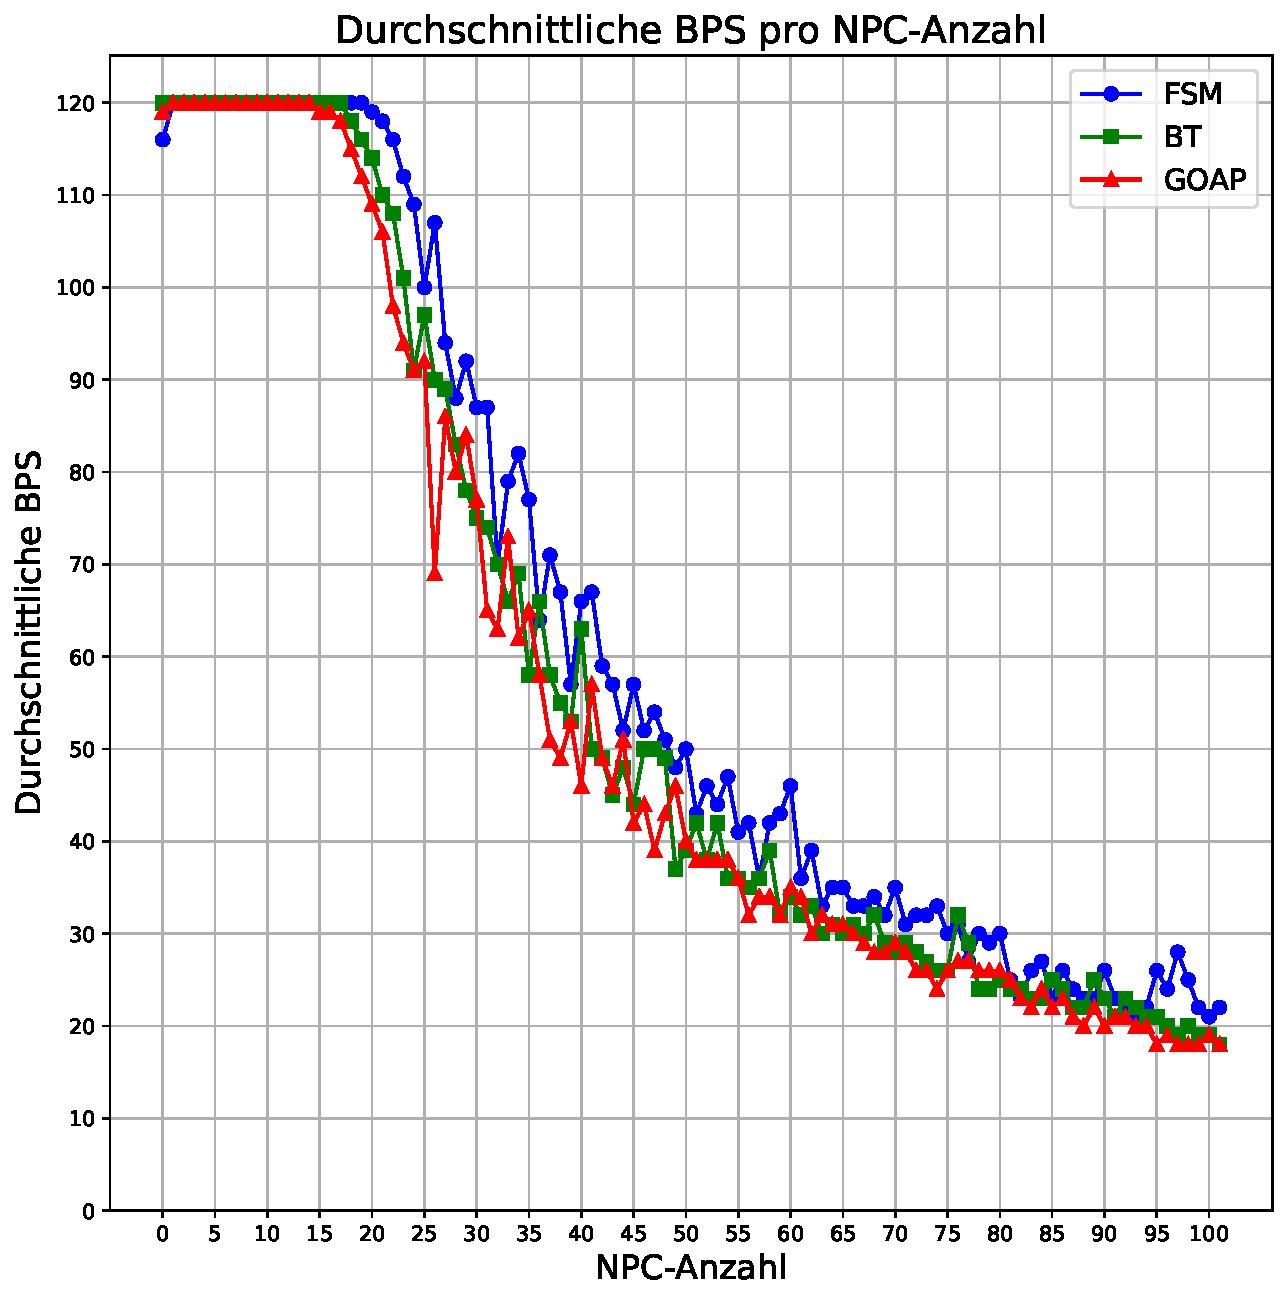
\includegraphics[width=14cm]{Vergleich/avg_fps.pdf}
	\captionsetup{justification=justified, format=plain}
  \caption{BPS-Performance Benchmark}
  \label{fig:bps benchmark}
\end{figure}

Die Abbildung \ref{fig:mem benchmark} veranschaulicht die Ergebnisse des Speicher-Benchmarks. Auch in diesem Fall erweist sich GOAP als ressourcenintensiv, jedoch bleibt der Speicherverbrauch laut dem Benchmark konstant. Es ist jedoch wichtig zu betonen, dass w\"{a}hrend der Implementierung GOAP mehrfach Speicherlecks aufgetreten sind, was auf eine h\"{o}here Empfindlichkeit dieses Systems hinweist.

\begin{figure}[h]
  \centering
  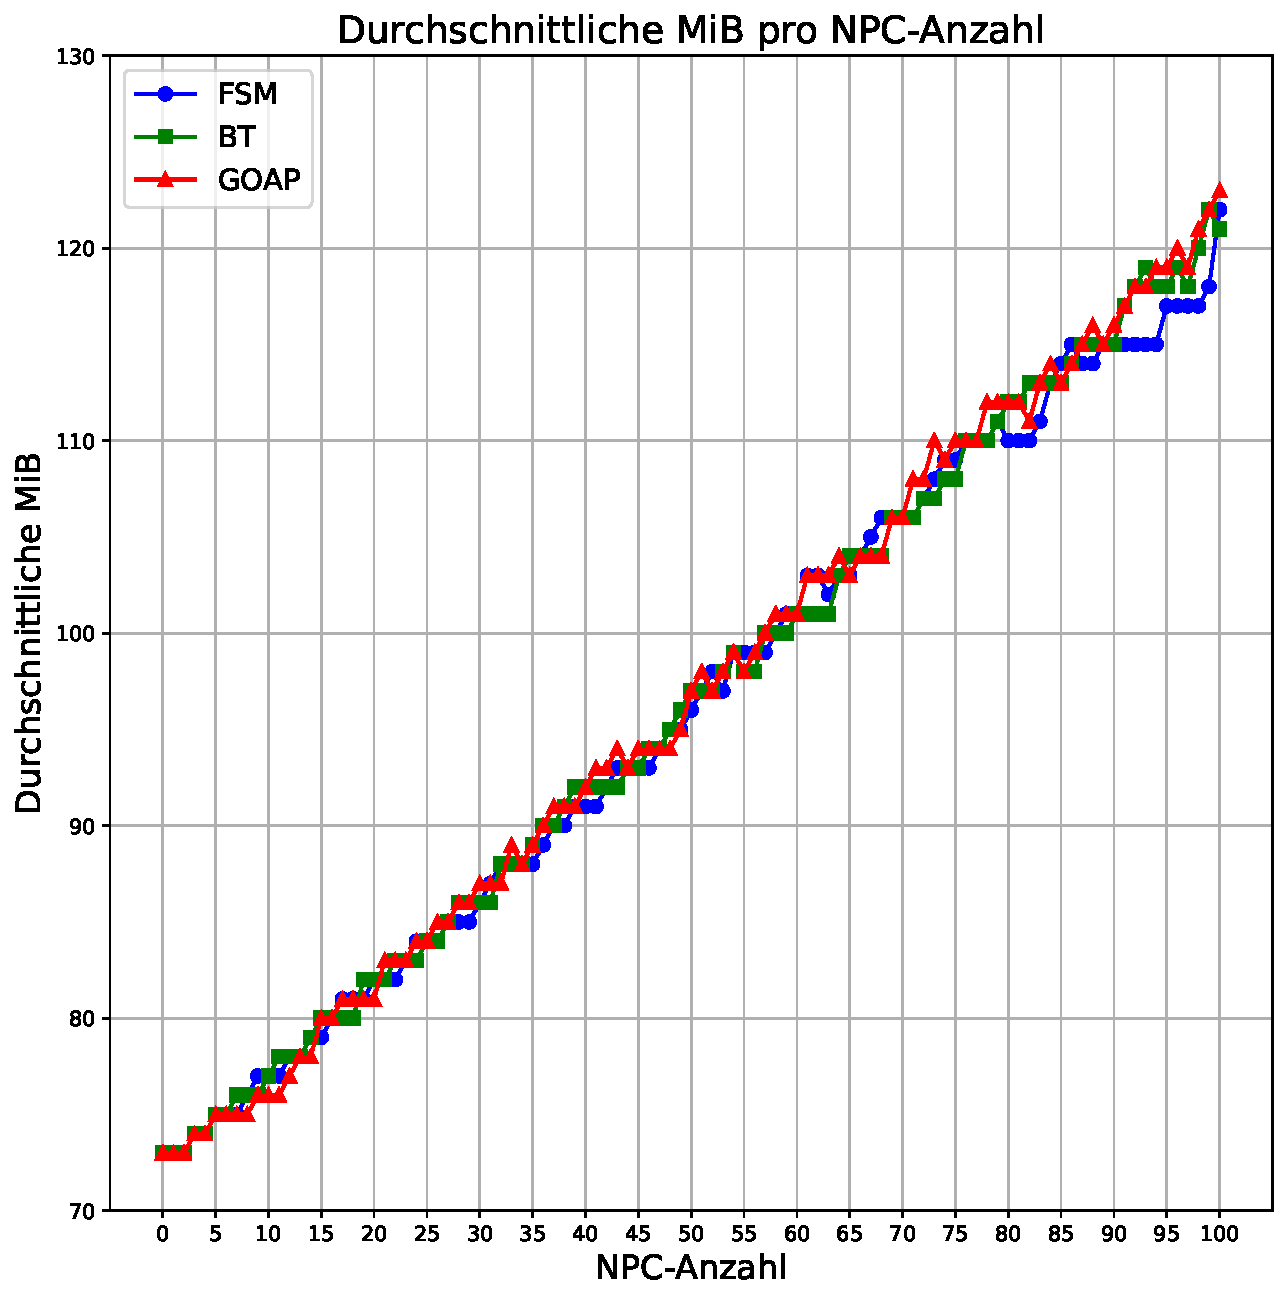
\includegraphics[width=14cm]{Vergleich/avg_mem.pdf}
	\captionsetup{justification=justified, format=plain}
  \caption{Speicher-Benchmark}
  \label{fig:mem benchmark}
\end{figure}


\clearpage


\section{Bewertung}
\label{chap:bewertung}

Die Wahl des Entscheidungssystems h\"{a}ngt stark von den Anforderungen des Projekts ab.

Eine FSM wird f\"{u}r einfache NPC-Logiken empfohlen. Sie ist von den anderen zwei Entscheidungssystem am einfachsten zu erlernen und in Godot umzusetzen. Will man aber komplexe NPC-Verhalten programmieren, so wird die Anzahl der Knoten wachsen, der FSM-Graph un\"{u}bersichtlicher und die Wartbarkeit wird schwieriger. Die Erweiterung durch weitere Knoten kann zur Anpassung der FSM f\"{u}hren und somit zu einem erh\"{o}hten Zeitaufwand. Das Debuggen ist jedoch durch die statische Natur der FSM vergleichsweise einfach, insbesondere wenn eine Visualisierung genutzt wird.

F\"{u}r mittlere bis komplexe NPC-Verhaltensweisen ist der BT zu empfehlen. Er ist in ihrer Funktionsweise komplexer als die FSM, hat aber viel Dokumentation zur Umsetzung, die in Godot ohne Schwierigkeiten m\"{o}glich ist. Die Skalierbarkeit und Debuggen des BT ist ebenfalls einfach. Es gibt außerdem interessante Studien, die die \textit{Usability} des BT erhöhen können (siehe Kapitel \ref{chap:bt sota}).

Will man komplexe NPC-Verhalten umsetzen, so ist GOAP die beste Wahl. Mit der komplexen Funktionsweise und eher mageren Dokumentation ist es schwierig, sich einzuarbeiten. In Bezug auf Skalierbarkeit \"{u}bertrifft GOAP die anderen Systeme, da neue Aktionen unabh\"{a}ngig voneinander existieren und nicht manuell verkn\"{u}pft werden m\"{u}ssen. Dies macht GOAP besonders anpassungsf\"{a}hig. Allerdings ist das Debuggen aufgrund der dynamischen Entscheidungen schwieriger. Eine m\"{o}gliche L\"{o}sung w\"{a}re die Visualisierung des Suchbaums, jedoch ist dies deutlich aufwendiger zu implementieren als bei FSM oder BT.

Die Tabelle \ref{tab:es vergleich tabelle} veranschaulicht die abschlie\ss{}ende Bewertung der Entscheidungssysteme mithilfe von Harvey Balls. Je voller der Harvey Ball, desto besser die Bewertung. Die Bewertungen basieren auf Vergleichen und Benchmarks.


\begin{table}[h]
  \caption{Tabellarische Bewertung}
  \label{tab:es vergleich tabelle}
  \centering
  \begin{tabular}{lccc}
    \toprule
    & FSM & BT & GOAP\\
    \midrule
		Erlernbarkeit & \harveyBallFull & \harveyBallThreeQuarter & \harveyBallHalf\\
    Implementierung	& \harveyBallFull  & \harveyBallThreeQuarter  & \harveyBallHalf\\
		NPC-Design & \harveyBallQuarter & \harveyBallThreeQuarter & \harveyBallFull\\
    Skalierbarkeit	& \harveyBallQuarter & \harveyBallHalf & \harveyBallFull\\
    Debugging	& \harveyBallHalf & \harveyBallThreeQuarter & \harveyBallQuarter\\
		Performance & \harveyBallFull & \harveyBallThreeQuarter & \harveyBallHalf\\
		Speicherverbrauch & \harveyBallFull & \harveyBallFull & \harveyBallThreeQuarter\\
    \bottomrule
  \end{tabular}
\end{table}